\documentclass[8pt]{article}
 
\usepackage[margin=.8in]{geometry} 
\usepackage{amsmath,amsthm,amssymb}
\usepackage{marvosym,enumerate,color,mathrsfs,graphicx,epstopdf}
\usepackage{enumitem}
%\setenumerate{listparindent=\parindent}
\def\cc{\color{blue}}
%\usepackage[dvipsnames]{xcolor}
\usepackage[normalem]{ulem}
\usepackage{bm}
\usepackage{mathtools}
\usepackage{mathrsfs}
\usepackage{verbatim}
\usepackage{tikz}
\usepackage[utf8]{inputenc}
\usepackage{hyperref}
\usepackage{courier}
\usepackage{fullpage}
\usepackage{graphicx}
\usepackage{float}
\hypersetup{
	%colorlinks,
	%citecolor=black,
	%filecolor=black,
	%linkcolor=blue,
	%urlcolor=black
}

\setlength{\footskip}{35pt}


%\usepackage{multirow}

%Line Numbering
\usepackage[mathlines]{lineno}
%\linenumbers
 
\newcommand{\N}{\mathbb{N}}
\newcommand{\Z}{\mathbb{Z}}
\newcommand{\R}{\mathbb{R}}
\newcommand{\C}{\mathbb{C}}
\newcommand{\Q}{\mathbb{Q}}
%\newcommand{\dell}{\partial}
\newcommand{\abs}[1]{\left\lvert{#1}\right\rvert}
\newcommand{\dx}{\mathrm{d}x}
\newcommand{\M}{\mathscr{M}}
\newcommand{\E}{\mathscr{E}}
\newcommand{\B}{\mathscr{B}}
\newcommand{\scr}[1]{\mathscr{#1}}
\newcommand{\Ns}{\mathscr{N}}
\newcommand{\nm}{\mathrel{\unlhd}}
\newcommand{\stcomp}[1]{{#1}^{\mathsf{c}}}
\newcommand{\closure}[1]{\overline{#1}}
\newcommand{\diam}{\operatorname{diam}}
\newcommand{\dist}{\operatorname{dist}}
\newcommand{\sgn}{\operatorname{sgn}}
\newcommand{\norm}[1]{\left\lVert{#1}\right\rVert}
\newcommand{\LR}[1]{\left\langle{#1}\right\rangle}

\theoremstyle{definition}
\newtheorem{theorem}{Theorem}
\newtheorem*{theorem*}{Theorem}
\newtheorem{lemma}[theorem]{Lemma}
\newtheorem{proposition}[theorem]{Proposition}
\newtheorem*{proposition*}{Proposition}
\newtheorem{definition}[theorem]{Definition}
\newtheorem*{definition*}{Definition}
\newtheorem{remark}[theorem]{Remark(s)}
\newtheorem*{remark*}{Remark(s)}
\newtheorem{corollary}[theorem]{Corollary}
\newtheorem*{corollary*}{Corollary}
\newtheorem{innerexercise}{Exercise}
\newenvironment{exercise}[1]
  {\renewcommand\theinnerexercise{#1}\innerexercise}
  {\endinnerexercise}

% Upper and lower integrals
%\def\upint{\mathchoice%
%    {\mkern13mu\overline{\vphantom{\intop}\mkern7mu}\mkern-20mu}%
%    {\mkern7mu\overline{\vphantom{\intop}\mkern7mu}\mkern-14mu}%
%    {\mkern7mu\overline{\vphantom{\intop}\mkern7mu}\mkern-14mu}%
%    {\mkern7mu\overline{\vphantom{\intop}\mkern7mu}\mkern-14mu}%
%  \int}
%\def\lowint{\mkern3mu\underline{\vphantom{\intop}\mkern7mu}\mkern-10mu\int}

\title{Numerical Analysis -- Homework 5}
\author{James Diffenderfer}
\date{\today}

%%%%%%%%%%%%%%%%%%%%%%%%%%%%%%%%%%%%%%
\begin{document}

\maketitle
%\tableofcontents

%\newpage

\begin{exercise}{1}
Numerically compute $$\int_{-1}^{1} \cos \left( 2x + \frac{1}{2} \right) dx$$ using
\begin{enumerate}
	\item [(a)] Composite Trapezoid rule
	\item [(b)] Composite Simpson's rule
	\item [(c)] Gaussian Quadrature.
\end{enumerate}
In each case, first use the error estimates given in class to find how large $n$ needs to be to ensure that the error in your computation is less that $10^{-5}$. Then perform the computation for that $n$ and confirm that your answer is within the estimated error.
\end{exercise}

\begin{proof}[Lower bound on $n$ for (a)]
For Composite Trapezoid rule we have that there exists an $\eta \in [-1, 1]$ such that
\begin{align*}
\left| \text{Error} \right| &= \left| \frac{(b - a)^3}{12 n^2} f''(\eta) \right| \\
&= \left| -4 \cos \left( 2 \eta + \frac{1}{2} \right) \frac{2^3}{12 n^2} \right| \\
&= \left| \cos \left( 2 \eta + \frac{1}{2} \right) \right| \left| \frac{8}{3 n^2} \right| \\
&\leq \frac{8}{3 n^2},
\end{align*}
where the last inequality follows from $| \cos x | \leq 1$, for all $x \in \mathbb{R}$. Hence, $| \text{Error} | \leq 10^{-5}$ provided that $$\frac{8}{3 n^2} \leq 10^{-5} \ \ \Longleftrightarrow \ \ 516.3977 \leq n.$$ Since $n$ should be an integer the computation will result in an error less than $10^{-5}$ for all $n \geq 517$.
\end{proof}

\begin{proof}[Lower bound on $n$ for (b)]
For Composite Simpson's rule we have that there exists an $\eta \in [-1, 1]$ such that
\begin{align*}
\left| \text{Error} \right| &= \left| \frac{(b - a)^5}{180 n^4} f^{(4)} (\eta) \right| \\
&= \left| 16 \cos \left( 2 \eta + \frac{1}{2} \right) \frac{2^5}{180 n^4} \right| \\
&= \left| \cos \left( 2 \eta + \frac{1}{2} \right) \right| \left| \frac{128}{45 n^4} \right| \\
&\leq \frac{128}{45 n^4}.
\end{align*}
Hence, $| \text{Error} | \leq 10^{-5}$ provided that $$\frac{128}{45 n^4} \leq 10^{-5} \ \ \Longleftrightarrow \ \ 23.09401077 \leq n.$$ Since $n$ should be an integer the computation will result in an error less than $10^{-5}$ for all $n \geq 24$.
\end{proof}

\begin{proof}[Lower bound on $n$ for (c)]
For Gaussian Quadrature we have that there exists an $\eta \in [-1, 1]$ such that
\begin{align*}
\left| \text{Error} \right| &= \left| \frac{f^{(2n)} (\eta)}{(2n)!} \right| \left| \int_{a}^{b} w^2 (x) dx \right| \\
&\leq \left| \frac{f^{(2n)} (\eta)}{(2n)!} \right| \left| \frac{2^{2n + 1} (n!)^4}{(2n + 1) ((2n)!)^2} \right| \\
&\leq \frac{2^{2n}}{(2n)!} \frac{2^{2n + 1} (n!)^4}{(2n + 1) ((2n)!)^2} \\
&= \frac{2^{4n + 1} (n!)^4}{(2n + 1) ((2n)!)^3}
\end{align*}
where the last inequality holds since $| f^{(2n)} (\eta) | = \left| 2^{2n} \cos \left( 2 \eta + \frac{1}{2} \right) \right| \leq 2^{2n}$. Since
\begin{center}
	\begin{tabular}{ | c | c |}
		\hline
		n & Error bound \\ \hline
		1 & \texttt{1.333333} \\ \hline
		2 & \texttt{0.118519} \\ \hline
		3 & \texttt{0.00406349} \\ \hline
		4 & \texttt{0.0000737141} \\ \hline
		5 & \texttt{8.27319 $\times$ 10e-7 } \\ \hline
	\end{tabular}
\end{center}
we conclude that the computation will result in an error less than $10^{-5}$ for all $n \geq 5$.
\end{proof}

\begin{proof}[Numerical Results]
The code for the computation of the integral using Composite Trapezoid Rule, Composite Simpson's Rule, and Gaussian Quadrature was written using python and is included on the final page of the assignment. Below is the output of program which verifies the claims presented for the required size of $n$ such that each method compute a value with error below the tolerance $10^{-5}$.\\

\texttt{--------------------------------- Exact Value ---------------------------------}\\
\indent \texttt{ Exact value of integral of cos(2x + .5) from -1 to 1: 0.797983565354 }\\

\texttt{----------------------------- Composite Trapezoid -----------------------------}\\
\indent \texttt{ Computed value with n = 517 steps: 0.797979584722}\\
\indent \texttt{ Computed error with n = 517 steps: 3.98063200735e-06 }\\

\texttt{----------------------------- Composite Simpson's -----------------------------}\\
\indent \texttt{ Computed value with n = 24 steps: 0.79798699741}\\
\indent \texttt{ Computed error with n = 24 steps: 3.43205640629e-06 }\\

\texttt{----------------------------- Gaussian Quadrature -----------------------------}\\
\indent \texttt{ Gaussian Quadrature value with n = 5 steps: 0.797984233643}\\
\indent \texttt{ Gaussian Quadrature error with n = 5 steps: 6.68288606454e-07 }\\
\end{proof}

\newpage

\begin{exercise}{2}
Let $T(a, b)$ and $T(a, (a + b)/2) + T((a + b)/2, b)$ be single and double applications of the Trapezoid rule to $\int_{a}^{b} f(x) \ dx$. Derive the approximate relation between $$\left| T(a, b) -  \left( T(a, (a + b)/2) + T((a + b)/2, b) \right) \right|$$ and $$\left| \int_{a}^{b} f(x) \ dx - \left( T(a, (a + b)/2) + T((a + b)/2, b) \right) \right|$$ used in adaptive Trapezoid quadrature.
\end{exercise}

\begin{proof}
Let $c = (a + b)/2$. By the error estimation for the Composite Trapezoid rule, we have that there exists a $\eta_0 \in [a, b]$ such that 
\begin{align}
\int_{a}^{b} f(x) dx = T(a, b) - \frac{h^3}{12} f''(\eta_0). \label{2.1}
\end{align}
Similarly, we have that for some $\eta_1 \in [a, c]$ and $\eta_2 \in [c, b]$
\begin{align}
\nonumber \int_{a}^{b} f(x) dx &= \int_{a}^{c} f(x) dx + \int_{c}^{b} f(x) dx \\
\nonumber &= T(a, c) - \frac{(h/2)^3}{12} f''(\eta_1) + T(c, b) - \frac{(h/2)^3}{12} f''(\eta_2) \\
&= T(a, c) + T(c, b) - \frac{(h/2)^3}{6} f''(\eta) \ \ \ \ \ \tag{exists $\eta \in (\eta_1, \eta_2)$ by I.V.T.} \\
&= T(a, c) + T(c, b) - \frac{1}{4} \cdot \frac{h^3}{12} f''(\eta). \label{2.2}
\end{align}
Hence, by assuming that $f''(\eta_0) \approx f''(\eta)$, combining (\ref{2.1}) and (\ref{2.2}) yields that
\begin{align}
\nonumber T(a, b) - (T(a, c) + T(c, b)) &= \frac{h^3}{12} f''(\eta_0) - \frac{1}{4} \cdot \frac{h^3}{12} f''(\eta) \\
\nonumber &= 3 \left[ \frac{1}{4} \cdot \frac{h^3}{12} f''(\eta) \right] \\
\nonumber &= 3 \left[ T(a,c) + T(c, b) - \int_{a}^{b} f(x) dx \right].
\end{align}
Thus, we conclude that $$\left| T(a, b) - (T(a, c) + T(c, b)) \right| = 3 \left| \int_{a}^{b} f(x) dx - (T(a,c) + T(c, b)) \right|,$$ assuming that the second derivative of $f$ is well-behaved on $[a, b]$.
\end{proof}





\begin{exercise}{3}
Let $h = (b - a)/3$, $x_0 = a$, $x_1 = a + h$, and $x_2 = b$. Find the degree of precision of the quadrature formula $$\int_{a}^{b} f(x) \ dx \approx \frac{9}{4} h f(x_1) + \frac{3}{4} h f(x_2).$$
\end{exercise}

\begin{proof}
Let $f_n (x) = x^n$, for $n \geq 0$. Observe, that 
\begin{align}
\int_{a}^{b} f_0 (x) dx &= b - a, \label{3.1} \\
\int_{a}^{b} f_1 (x) dx &= \frac{b^2 - a^2}{2}, \label{3.2} \\
\int_{a}^{b} f_2 (x) dx &= \frac{b^3 - a^3}{3}, \label{3.3} \\
\int_{a}^{b} f_3 (x) dx &= \frac{b^4 - a^4}{4}, \label{3.7}
\end{align}
and that
\begin{align}
\nonumber \frac{9}{4} h f_0(x_1) + \frac{3}{4} h f_0(x_2) &= \frac{9}{4} \frac{(b - a)}{3} + \frac{3}{4} \frac{(b - a)}{3} \\
&= b - a, \label{3.4}
\end{align}
\begin{align}
\nonumber \frac{9}{4} h f_1(x_1) + \frac{3}{4} h f_1(x_2) &= \frac{9}{4} \frac{(b - a)}{3} \left( a + \frac{b - a}{3} \right) + \frac{3}{4} \frac{(b - a)}{3} b \\
\nonumber &= \frac{1}{4} (b - a) \left[ 2a + 2b \right] \\
&= \frac{b^2 - a^2}{2}, \label{3.5}
\end{align}
\begin{align}
\nonumber \frac{9}{4} h f_2(x_1) + \frac{3}{4} h f_2(x_2) &= \frac{9}{4} \frac{(b - a)}{3} \left( a + \frac{b - a}{3} \right)^2 + \frac{3}{4} \frac{(b - a)}{3} b^2 \\
\nonumber &= \frac{1}{4} (b - a) \left[ \frac{(2a + b)^2}{3} + b^2 \right] \\
\nonumber &= \frac{1}{4} (b - a) \left[ \frac{4 a^2 + 4ab + 4b^2}{3} \right] \\
&= \frac{b^3 - a^3}{3}. \label{3.6}
\end{align}
\begin{align}
\nonumber \frac{9}{4} h f_3(x_1) + \frac{3}{4} h f_3(x_2) &= \frac{9}{4} \frac{(b - a)}{3} \left( a + \frac{b - a}{3} \right)^2 + \frac{3}{4} \frac{(b - a)}{3} b^3 \\
\nonumber &= \frac{1}{4} (b - a) \left[ \frac{(2a + b)^3}{9} + b^3 \right] \\
&= \frac{1}{4} (b - a) \left[ \frac{8 a^3 + 12 a^2 b + 6 a b^2 + 10 b^3}{9} \right]. \label{3.8}
\end{align}
Since the expressions for (\ref{3.1}) and (\ref{3.4}) are equal, (\ref{3.2}) and (\ref{3.5}) are equal, (\ref{3.3}) and (\ref{3.6}) are equal, but (\ref{3.7}) and (\ref{3.8}) are not equal we conclude that this quadrature formula has degree of precision 2.
\end{proof}


\begin{exercise}{4}
Derive the error term in Simpson's rule by assuming that
\begin{align*}
\int_{a}^{b} f(x) \ dx = \frac{b - a}{6} \left( f(a) + 4 f \left( \frac{a + b}{2} \right) + f(b) \right) + k f^{(4)} (\eta) \tag{$\ast$}
\end{align*}
and finding $k$ by using the formula for $f(x) = x^4$. 
\end{exercise}

\begin{proof}
Using $f(x) = x^4$ the right hand side of ($\ast$) simplifies to
\begin{align}
\nonumber \frac{b - a}{6} \left( a^4 + 4 \left( \frac{a + b}{2} \right)^4 + b^4 \right) + 24 k &= \frac{b - a}{6} \cdot \frac{1}{4} (5 a^4 + 4 a^3 b + 6 a^2 b^2 + 4 a b^3 + 5 b^4) + 24 k.
\end{align}
Since the left hand side of ($\ast$) is equal to $(b^5 - a^5)/5$ we get that
\begin{align*}
k &= \frac{1}{24} \left[ \frac{b^5 - a^5}{5} - \frac{b - a}{24} (5 a^4 + 4 a^3 b + 6 a^2 b^2 + 4 a b^3 + 5 b^4) \right] \\
&= \frac{b - a}{24} \left[ \frac{1}{5} (a^4 + a^3 b + a^2 b^2 + a b^3 + b^4) - \frac{1}{24} (5 a^4 + 4 a^3 b + 6 a^2 b^2 + 4 a b^3 + 5 b^4) \right] \\
&= \frac{b - a}{24} \cdot \frac{1}{120} (-a^4 + 4 a^3 b - 6 a^2 b^2 + 4 a b^3 - b^4) \\
%&= \frac{b - a}{24} \cdot \frac{- (b - a)^4}{120} \\
&= - \frac{(b - a)^5}{2880} \\
&= - \frac{1}{90} \left( \frac{b - a}{2} \right)^5,
\end{align*}
the desired result.
\end{proof}

\end{document}

% Figure Stuff
\begin{figure}[H]
	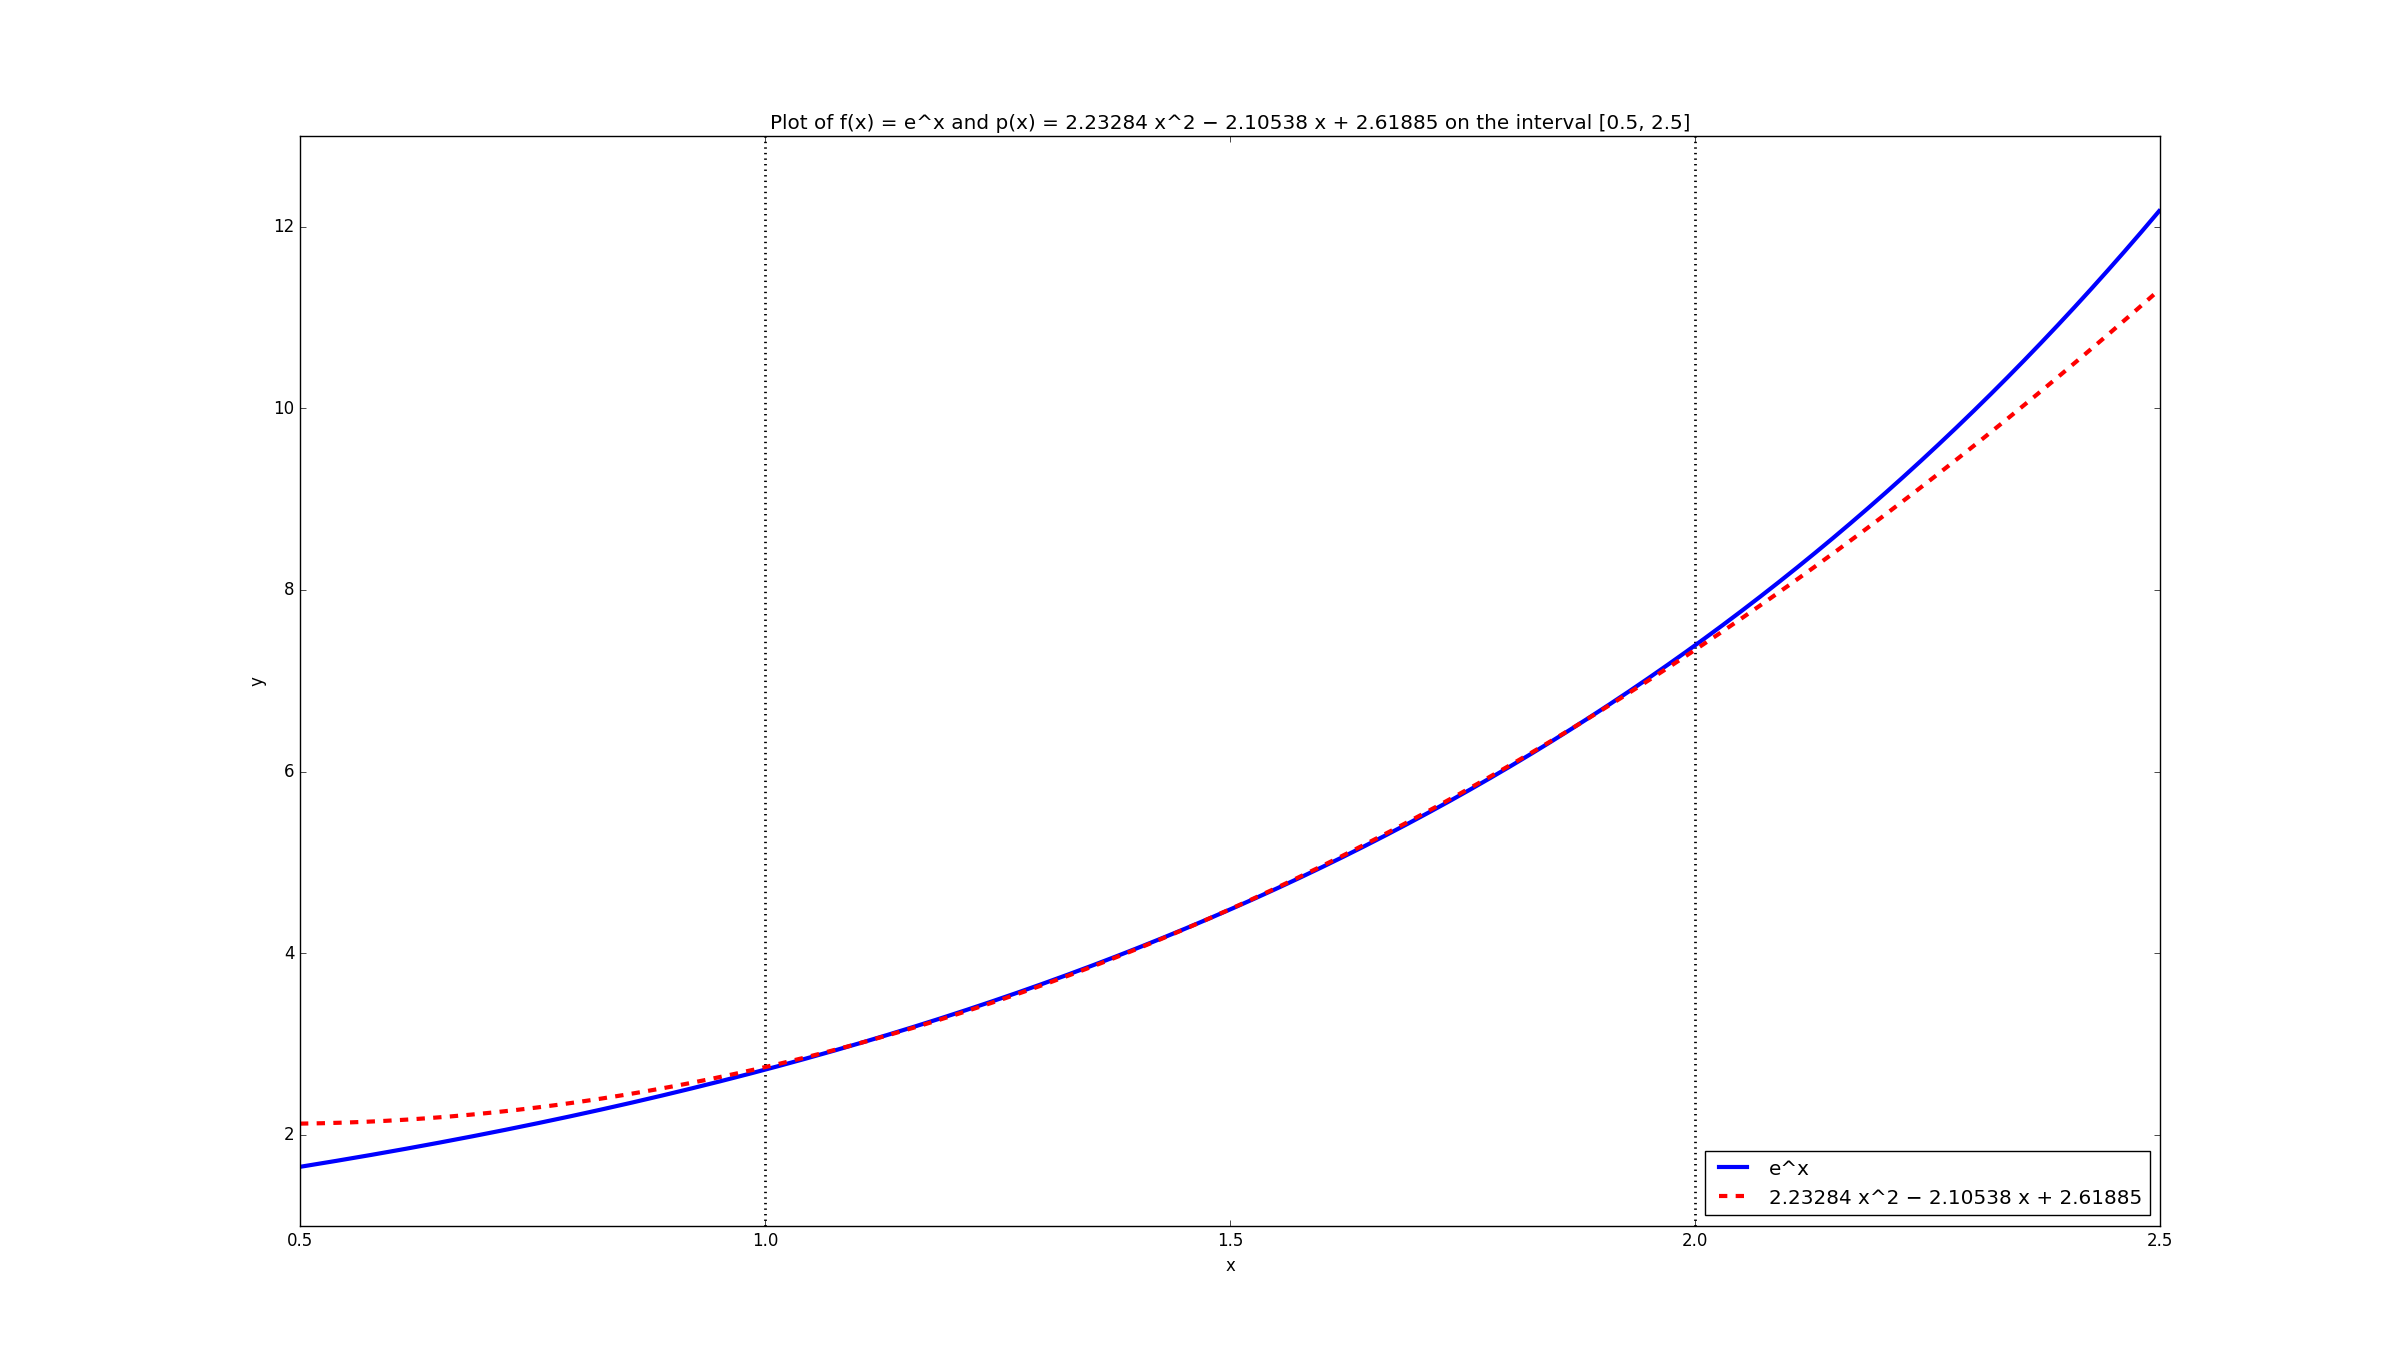
\includegraphics[trim={6cm, 0, 5cm, 2cm}, clip, width=\textwidth]{ortho_plot.png}
	\vspace{-10mm}
	\caption{Plot of $f(x) = e^x$ (solid line) and $p(x) = 2.23284 x^2 - 2.10538 x + 2.61885$ (dashed line), the polynomial constructed in 2 (a).}
	\label{Figure 1}
\end{figure}

% Stuff for wolfram alpha to simplify
(\frac{1}{4} n^2 + \frac{1}{4} n) (\frac{5}{4} n^2 + \frac{13}{4} n + \varepsilon) - n (\frac{5}{12} n^3 + \frac{9}{8} n^2 + \frac{17}{24} n + \delta)

(\frac{1}{4} n^2 + \frac{1}{4} n)^2 - n (\frac{1}{12} n^3 + \frac{1}{8} n^2 + \frac{1}{24} n)

% Incorrect work for #3
Hence $$\phi_0 (t) = \sqrt{1/2}, \ \ \ \phi_1 (t) = \sqrt{3/2} \ (t + 2), \ \ \ \text{and} \ \ \ \phi_2 (t) = \sqrt{5/8} \ (3t^2 + 12 t + 11).$$ Now by defining $f(t) = e^{t + 2}$ we have $$p_2 (t) = \langle f(t), \phi_0 \rangle \phi_0 + \langle f(t), \phi_1 \rangle \phi_1 + \langle f(t), \phi_2 \rangle \phi_2.$$ Since $$\langle f(t), \phi_0 \rangle = e^2 \sqrt{\frac{1}{2}} \int_{-1}^{1} e^t \approx 12.28050385,$$ $$\langle f(t), \phi_1 \rangle = e^2 \sqrt{\frac{3}{2}} \int_{-1}^{1} e^t (t + 2) = 2 e^3 \sqrt{\frac{3}{2}} \approx 49.19931667,$$ and $$\langle f(t), \phi_2 \rangle = e^2 \sqrt{\frac{5}{8}} \int_{-1}^{1} e^t (3t^2 + 12t + 11) = e^2 \left( 14 e - \frac{2}{e} \right) \sqrt{\frac{5}{8}} \approx 218.0081755$$ we have that 
\begin{align*}
p_2 (t) = 12.28050385 \sqrt{\frac{1}{2}} + 49.19931667 (t + 2) \sqrt{\frac{3}{2}} + 218.0081755 (3t^2 + 12 t + 11) \sqrt{\frac{5}{8}} \\
&= 
\end{align*}

% Some unused code
# Generate data set {(x_1, y_1), ..., (x_20, y_20)}
    for k in range(1, m + 1):
        # Initialize x_k = k/2
        x.append(k/2)

        # Initialize eps_k as a random number uniformly distributed in [-2, 2]
        epsilon = np.random.uniform(-2, 2)

        # Set y_k = 5x_k + 2 + eps_k
        y.append(5*k/2 + 2 + epsilon)
